\documentclass{llncs}

\usepackage{graphicx}

\begin{document}

\pagestyle{empty}

\mainmatter

\title{An Underapproximation Refinement Based Concurrent Program Verification Tool}

%TODO: add authors

%TODO: add email and institute of authors

\maketitle

\begin{abstract}
\label{sect:abstract}
%should be at least 70 words and at most 150
We have developed a tool to verify safety properties of concurrent programs in symbolic bounded model checking setting. Given an ANSI-C or C++ shared memory concurrent program and safety properties specified as assert statements the tool underapproximates dataflow of the program using likely invariants. The likely invariants are generated by dynamic analysis and added as constraints in given program. This program is verified on a SAT-based bounded model checker. Further, the tool performs refinement of underapproximated dataflow using UNSAT proof. Our technique is applicable for different encoding techniques used to represent concurrent programs. We evaluate the performance of the tool on two encodings and multiple benchmarks.
\end{abstract}

\section{Introduction}
\label{sect:introduction}
Automatic verification of concurrent programs written in low level languages like ANSI-C is an important task as multi-core architecture is gaining widespread adoption. The difficulty in development of programs due to concurrency and different memory models of processors adds to the importance of such a tool. However, verification of concurrent programs is proven to be harder than sequential programs\cite{rama}. Sequentialization is an approach to overcome this difficulty by considering a restricted model. In sequentialization a concurrent program is transformed to an equivalent nondeterministic sequential program by restricting the dataflow of shared memory operations. Apart from tackling the hardness, sequentialization enables us to use existing sequential analysis tools on concurrent programs.

%TODO: do we need to add references to tools using CBA?
Context-bounded analysis\cite{kiss,lal} is the earliest sequentialization technique where number of context switches is bounded.\cite{alglave} is another approach which bounds the number of loop unwindings and then performs symbolic bounded model checking. In \cite{alglave} a concurrent program is transformed to a formula consisting of two conjuncts. The first conjunct encodes control and data flow of individual threads and the second conjunct encodes possible interaction between shared memory instructions as partial orders. Recently memory unwinding technique\cite{tomasco}\cite{anand} has been proposed where the number of shared memory writes are bounded. In \cite{tomasco}\cite{anand} source-to-source transformation of a concurrent program to a sequential nondeterministic program is performed. This nondeterministic sequential program is passed to a symbolic bounded model checker like CBMC\cite{cbmc}. 

%TODO: expand rf of alglave
The nondeterminism in \cite{alglave}\cite{tomasco}\cite{anand} is introduced to represent every possible shared memory interactions allowed in a memory model. In \cite{anand} shared memory writes are nondeterministically assigned timestamps to represent happens before relation (a write \textit{$w_1$} with timestamp \textit{$t_{w_1}$} preceedes another write \textit{$w_2$} with timestamp \textit{$t_{w_2}$} when \textit{$t_{w_1}$} $<$ \textit{$t_{w_2}$}). Shared memory reads are nondeterministically mapped to shared memory writes as shown in Fig.~\ref{code:anand_read}. Here \textit{read\_y} corresponds to read instruction of variable \textit{$y$}. It first selects an index of timestore(an array of timestamps of writes) ranging over index of latest write to maximum number of writes allowed, then updates its datastructures and finally returns symbolic value corresponding to write it has selected. The length of possible range of indices, which corresponds to possible set of writes, is a major factor in determining the state space. In \cite{alglave} a partial order relation named \textit{rf} is used.

%TODO: add information about how this will optimise rf after "find assert violation"
We observe that instead of starting with all possible writes we can start with a subset of writes and then increase the number of writes considered for only those instructions which are relevant to the property. For instance, consider the example shown in Fig.~\ref{code:motivate}. Here two threads are executing functions \textit{$t1,t2$} concurrently and using \textit{$x,y$} which are global variables. This program is not safe as lines \textit{$4-9$} of \textit{t2} are wrongly considered as atomic. Consider an execution where the value of \textit{$y$} has become \textit{$NUM-1$} and currently thread running \textit{$t1$} has execution context. \textit{$t1$} executes lines \textit{$2-6$} setting \textit{$y$} to \textit{$NUM$} after which thread executing \textit{$t2$} gets the execution context. \textit{$t2$} executes lines \textit{$3-7$} after which \textit{$t1$} is executed again. In this execution context thread executing \textit{$t1$} completes its execution updating \textit{$x$}. Following this, thread executing \textit{$t2$} and assert in line \textit{$9$} is violated as value of \textit{$x$} has changed from what it observed at line \textit{$6$}. For this program the encoding of \textit{$read\_y$} of \cite{anand} considers writes of \textit{$t1$}(line \textit{$10$}) and \textit{$t2$}(line \textit{$8$}). However, by considering only local write (line \textit{$10$} of \textit{$t1$}) for reads of \textit{$t1$} we can still find the assert violation. 
%
\medskip
\noindent
\label{code:anand_read}
\begin{figure}
\begin{verbatim}
1 int read_y() 
2 { unsigned short loc=*;
3   assume(loc_y <= loc < MAXW_y &&
4          ts_y[loc+1] > ct);
5   loc_y = loc;
6   if (ct<ts_y[loc]) ct=ts_y[loc];
7   return value_y[loc];}
\end{verbatim}
\caption{Shared memory read encoding from \cite{anand}}
\label{code:anand_enc}
\end{figure}
%
\noindent
\begin{figure}
\begin{verbatim}
  int x = 0, y = 0;
1 void * t1() {                1 void * t2() {
2   while (read_y() < NUM) {   2  int t, tmp1, tmp2;
3     int tmp1, tmp2;          3  while (read_y() < NUM) { }
4     //y = y + 1              4  t = read_y();
5     tmp1 = read_y();         5  //y = x + y;
6     write_y(tmp1 + 1);       6  tmp1 = read_x();
7     //x = x + y;             7  tmp2 = read_y();
8     tmp1 = read_x();         8  write_y(tmp1 + tmp2);
9     tmp2 = read_y();         9  assert(read_y() == t + read_x());  
10    write_y(tmp1 + tmp2);    10 }}
11  }}
\end{verbatim}
\caption{Motivating Example}
\label{code:motivate}
\end{figure}
%

Given a program which can be represented as $L_C \cap L_D$, where $L_C$ is control flow and dataflow of local memory and $L_D$ is dataflow of shared memory, our tool starts with $L_C \cap L_{D'}$, where $L_{D'} \subseteq L_D$, and either proves that $L_D \setminus L_{D'}$ is irrelevant to the property or infeasible, or refines $L_{D'}$ towards $L_D$. 

\section {Implementation} 
\label{sect:implementation}

\begin{figure}
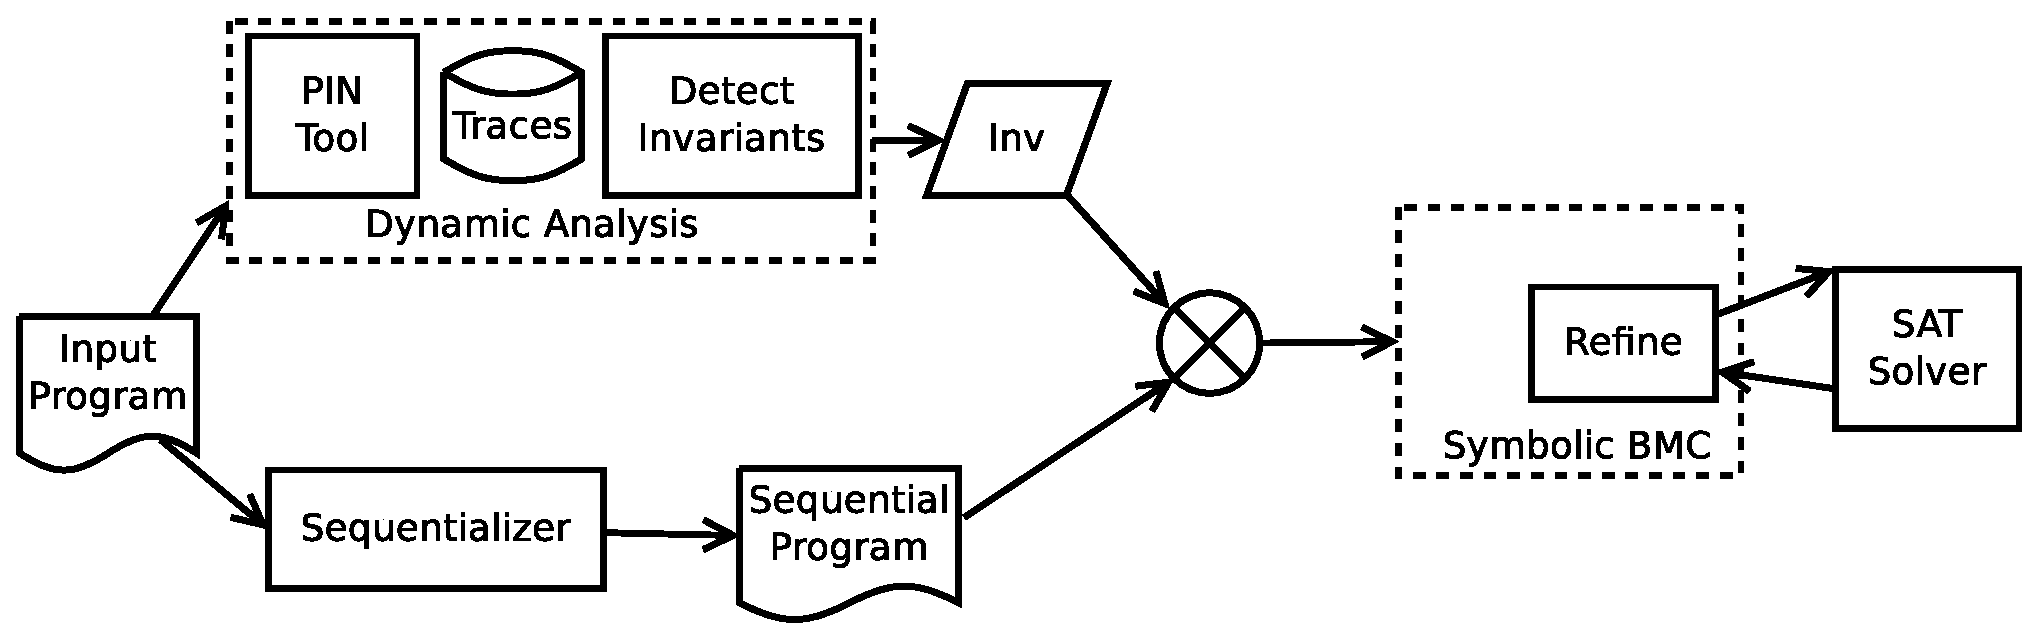
\includegraphics[scale=0.35]{design.eps}
\centering
\caption{Design of the tool}
\label{fig:design}
\end{figure}

\subsection {Likely Invariant Generation}
\label{sect:inv_gen}
The input concurrent program is instrumented to track shared memory instructions by using a PIN\cite{pin} tool.The instrumented program is executed under PIN and execution traces, which are sequences of instruction address, operand address and thread index, are collected. These traces are analysed to generate three classes of likely invariants following \cite{defuse}. Thus generated invariants are added as constraints in the program depending on encoding. 

\subsection {Adding likely inavriants as constraints}
\label{sect:inv_const}
The above generated invariants are added as constraints 
\subsection {Refinement}
\label{sect:refinement}

\section {Experiments}
\label{sect:experiments}

\section {Conclusion and Future Work}
\label{sect:conclusion}

\begin{thebibliography}{4}
%
\bibitem{rama}
Ramalingam G. Context-sensitive synchronization-sensitive analysis is undecidable. 
ACM Transactions on Programming languages and Systems (TOPLAS). 2000 Mar 1;22(2):416-30.
%
\bibitem{kiss}
Qadeer S, Wu D. KISS: keep it simple and sequential. Acm sigplan notices. 2004 Jun 9;39(6):14-24.
%
\bibitem{lal}
Lal A, Reps T. Reducing concurrent analysis under a context bound to sequential analysis. 
Formal Methods in System Design. 2009 Aug 1;35(1):73-97.
%
\bibitem{alglave}
Alglave J, Kroening D, Tautschnig M. 
Partial orders for efficient bounded model checking of concurrent software. 
In International Conference on Computer Aided Verification 2013 Jul 13 (pp. 141-157). 
Springer Berlin Heidelberg.
%
\bibitem{tomasco}
Tomasco E, Inverso O, Fischer B, La Torre S, Parlato G. 
Verifying concurrent programs by memory unwinding. 
In International Conference on Tools and Algorithms for the Construction and Analysis of 
Systems 2015 Apr 11 (pp. 551-565). Springer Berlin Heidelberg.
%
%TOO: Modify bibtex to actual Anand's bibtex
\bibitem{anand}
Anand Yeolekar, Kumar Madhukar, Dipali Bhutada, Venkatesh R.
Sequentialization Using Timestamps.
In International Conference on Tools and Algorithms for the Construction and Analysis of 
Systems 2015 Apr 11 (pp. 551-565). Springer Berlin Heidelberg.
%
\bibitem{cbmc}
Kroening D, Tautschnig M. 
CBMC - C bounded model checker. 
In International Conference on Tools and Algorithms for the Construction and Analysis of Systems 2014 Apr 5 (pp. 389-391). Springer Berlin Heidelberg.
%
\bibitem{cseq}
Fischer B, Inverso O, Parlato G. 
CSeq: A concurrency pre-processor for sequential C verification tools. 
In Automated Software Engineering (ASE), 2013 IEEE/ACM 28th International Conference on 2013 Nov 11 (pp. 710-713). IEEE.
%
\bibitem{pin}
Luk CK, Cohn R, Muth R, Patil H, Klauser A, Lowney G, Wallace S, Reddi VJ, Hazelwood K. 
Pin: building customized program analysis tools with dynamic instrumentation. 
In Acm sigplan notices 2005 Jun 12 (Vol. 40, No. 6, pp. 190-200). ACM.
%
\bibitem{defuse}
Shi Y, Park S, Yin Z, Lu S, Zhou Y, Chen W, Zheng W. 
Do I use the wrong definition?: DeFuse: definition-use invariants for detecting concurrency and sequential bugs. 
In ACM Sigplan Notices 2010 Oct 17 (Vol. 45, No. 10, pp. 160-174). ACM.
%
\end{thebibliography}

\end{document}
